\documentclass{article}

\def\npart {II}
\def\nyear {2017}
\def\nterm {Michaelmas}
\def\nlecturer{Dr C. Brookes}
\def\ncourse{Galois Theory}
\ifx \nauthor\undefined
  \def\nauthor{Bhavik Mehta}
\else
\fi

\author{Based on lectures by \nlecturer \\\small Notes taken by \nauthor}
\date{\nterm\ \nyear}
\title{Part \npart\ -- \ncourse}

\usepackage[utf8]{inputenc}
\usepackage{amsmath}
\usepackage{amsthm}
\usepackage{amssymb}
\usepackage{enumerate}
\usepackage{mathtools}
\usepackage{graphicx}
\usepackage[dvipsnames]{xcolor}
\usepackage{tikz}
\usepackage{wrapfig}
\usepackage{centernot}
\usepackage{float}
\usepackage{braket}
\usepackage[hypcap=true]{caption}
\usepackage{enumitem}
\usepackage[colorlinks=true, linkcolor=mblue]{hyperref}
\usepackage[nameinlink,noabbrev]{cleveref}
\usepackage{nameref}
\usepackage[margin=1.5in]{geometry}

% Theorems
\theoremstyle{definition}
\newtheorem*{aim}{Aim}
\newtheorem*{axiom}{Axiom}
\newtheorem*{claim}{Claim}
\newtheorem*{cor}{Corollary}
\newtheorem*{conjecture}{Conjecture}
\newtheorem*{defi}{Definition}
\newtheorem*{eg}{Example}
\newtheorem*{ex}{Exercise}
\newtheorem*{fact}{Fact}
\newtheorem*{law}{Law}
\newtheorem*{lemma}{Lemma}
\newtheorem*{notation}{Notation}
\newtheorem*{prop}{Proposition}
\newtheorem*{question}{Question}
\newtheorem*{rrule}{Rule}
\newtheorem*{thm}{Theorem}
\newtheorem*{assumption}{Assumption}

\newtheorem*{remark}{Remark}
\newtheorem*{warning}{Warning}
\newtheorem*{exercise}{Exercise}

% \newcommand{\nthmautorefname}{Theorem}

\newtheorem{nthm}{Theorem}[section]
\newtheorem{nlemma}[nthm]{Lemma}
\newtheorem{nprop}[nthm]{Proposition}
\newtheorem{ncor}[nthm]{Corollary}
\newtheorem{ndef}[nthm]{Definition}

% Special sets
\newcommand{\C}{\mathbb{C}}
\newcommand{\N}{\mathbb{N}}
\newcommand{\Q}{\mathbb{Q}}
\newcommand{\R}{\mathbb{R}}
\newcommand{\Z}{\mathbb{Z}}

\newcommand{\abs}[1]{\left\lvert #1\right\rvert}
\newcommand{\norm}[1]{\left\lVert #1\right\rVert}
\renewcommand{\vec}[1]{\boldsymbol{\mathbf{#1}}}

\let\Im\relax
\let\Re\relax

\DeclareMathOperator{\Im}{Im}
\DeclareMathOperator{\Re}{Re}
\DeclareMathOperator{\id}{id}

\definecolor{mblue}{rgb}{0., 0.05, 0.6}


% preamble
\setcounter{section}{-1}
\usepackage{tkz-euclide}
\usepackage{xfrac}
\usetkzobj{all}

\DeclareMathOperator{\Aut}{Aut}
\DeclareMathOperator{\Hom}{Hom}
\DeclareMathOperator{\Root}{Root}
\DeclareMathOperator{\chara}{char}
\DeclareMathOperator{\Tr}{Tr}

\newtheorem{nexample}[nthm]{Example}
\newtheorem{nremark}[nthm]{Remark}
\newcommand{\F}{\mathbb{F}}

\newtheorem{manualinner}{}
\newenvironment{manual}[1]{%
    \renewcommand\themanualinner{#1}%
    \manualinner
}{\endmanualinner}
% and here we go!

\begin{document}
\maketitle

\tableofcontents

% lecture 1

\section{Introduction}
The primary motivation of this course is to study the solutions of polynomial equations in one variable to wander whether there is a formula involving roots, a solution by radicals.
Quadratics were typically studied in school, while the solution in radicals for cubics and quartics has been known for a long time and studied in particular in 1770 by Lagrange.

In 1799, Ruffini claimed that there were some quintics that can't be solved by radicals, that is, there is no general formula, but it took until 1824 before Abel used existing ideas about permutations to produce the first accepted proof of insolubility, before dying in 1829.
Galois' main contribution was in 1831, when he gave the first explanation as to why some polynomials are soluble by radicals and others are not.
He made use of the group of permutations of the roots of a polynomial, and realised in particular the importance of \emph{normal} subgroups.

Galois' work was not known generally in his lifetime - it was only published by Liouville in 1846, who realised that it tied in well with the work of Cauchy on permutations.
Galois had submitted his work for various competitions and for entry into the Ecole Polytechnique in Paris.
Unfortunately Galois died in a duel in 1832, leaving a six and a half page letter indicating his thoughts about the future development of his theory.

\subsection{Course overview}
Most of this course is Galois Theory, but presented in a more modern fashion- in terms of field extensions.
Recall from GRM that if $f(t)$ is an irreducible polynomial in $k[t]$ where $k$ is a field, then $k[t]/(f(t))$ is a field, where $(f(t))$ denotes the ideal of $k[t]$ generated by $f(t)$, and this new field contains $k$.
In this way, we can see the field $k[t]/(f(t))$ as a field extension of $k$.

% Galois' papers have been studied by Peter Neumann:
% The math writings of Evariste Galois, European Math Soc
% Different books: I. Steward Galois Theory, (something) and Hall
% contains a historcal introduction and covers almost all the syllabus.
% Artin Galois Theory
% Van der Waerden Modern Algebra (covers a lot more than Galois theory)
% Lang Algebra (late editions are preferred, covers a lot of algebra)
% Kaplansky Fields and Rings

\paragraph{Prerequisites} Quite a lot of the Groups, Rings and Modules course, but no modules except in one place where it's useful to know the structure of finite abelian groups.
The DPMMS website has a Galois Theory page with a long history of example sheets and notes, in particular see Tony Scholl's 2013-4 course page.
\clearpage

\section{Field Extensions}
\begin{ndef}\hypertarget{def:fieldExt}
    A \textbf{field extension} $K \leq L$ is the inclusion of a field $K$ into another field $L$ with the same $0$, $1$, and where the restriction of $+$ and $.$ (in L) to $K$ gives the $+$ and $.$ of $K$.
\end{ndef}

\begin{eg}
    \leavevmode
    \begin{enumerate}[label=(\roman*)]
        \item $\Q \leq \R$
        \item $\R \leq \C$
        \item $\Q \leq \Q(\sqrt{2}) = \Set{\lambda + \mu \sqrt{2} | \lambda, \mu \in \Q}$
        \item $\Set{\lambda + \mu i | \lambda, \mu \in \Q} = \Q(i) \leq \C$
    \end{enumerate}
\end{eg}

Suppose $K \leq L$ is a \hyperlink{def:fieldExt}{field extension}. Then $L$ is a $K$-vector space using the addition from the field structure and scalar multiplcation given by the multiplication in the field $L$.

\begin{ndef}\hypertarget{def:degreeOfFieldExt}
    The \textbf{degree} of $L$ over $K$ is $\dim_K L$, the $K$-vector space dimension of $L$. This may not be finite. We typically denote this by $\abs{L:K}$.
    If $\abs{L:K} < \infty$, then the extension is \textbf{finite}, otherwise the extension is \textbf{infinite}.
\end{ndef}

\begin{eg}\leavevmode
    \begin{enumerate}[label=(\roman*)]
        \item $\abs{\C:\R} = 2$, with $\R$-basis $1, i$
        \item $\abs{\Q(i):\Q} = 2$, with $\Q$-basis $1, i$
        \item $\Q \leq \R$ is an infinite extension.
    \end{enumerate}
\end{eg}

\begin{nthm}[Tower law]\label{thm:towerLaw}
    Suppose $K \leq L \leq M$ are field extensions. Then $\abs{M:K}$ = $\abs{M:L}\abs{L:K}$.
\end{nthm}
\begin{proof}
    Assume that $\abs{M:L} < \infty$, and $\abs{L:K} < \infty$.
    Take an $L$-basis of $M$, given by $\Set{f_1, \dotsc, f_b}$, and a $K$-basis of $L$ given by $\Set{e_1, \dotsc, e_a}$.
    Take $m \in M$, so $m = \sum_{i=1}^b \mu_i f_i$ for some $\mu_i \in L$.
    Similarly, $\mu_i = \sum_{j=1}^a \lambda_{ij} e_j$ for some $\lambda_{ij} \in K$, so

    \begin{equation*}
        m = \sum_{i=1}^b \sum_{j=1}^a \lambda_{ij} e_j f_i
    \end{equation*}
    Thus $\Set{e_j f_i | 1 \leq j \leq a, 1 \leq i \leq a}$ span $M$.

    Linear independence:
    It's enough to show that if $0 = m = \sum \sum \lambda_{ij} e_j f_i$ then $\lambda_{ij}$ are all zero.
    However if $m = 0$ the linear independence of $f_i$ forces each $\mu_i = 0$.
    Then the linear indepedence of $e_j$ forces $\lambda_{ij}$ all to be zero, as required.
\end{proof}

The tower law will not be proved for \hyperlink{def:degreeOfFieldExt}{infinite} extensions, but observe that if $M$ is an infinite extension of $L$ then it is an infinite extension of $K$, and similarly if $L$ is an infinite extension of $K$ then the larger field $M$ must also be an infinite extension of $K$.

\subsection{Motivatory Example}
Observe $\Q \leq \Q\left(\sqrt{2}\right) \leq \Q\left(\sqrt{2}, i\right)$
\begin{enumerate}[label=(\roman*)]
    \item $\Q\left(\sqrt{2}\right)$ has basis $1, \sqrt{2}$ over $\Q$.
    \item $\Q\left(\sqrt{2}, i\right)$ has basis $1, i$ as a $\Q\left(\sqrt{2}\right)$--vector space.
    \item $\Q\left(\sqrt{2}, i\right)$ has basis $1, \sqrt{2}, i, i\sqrt{2}$ over $\Q$.
\end{enumerate}
\begin{equation*}
    \abs{\Q\left(i, \sqrt{2}\right):\Q} = 4 = 2 \cdot 2 = \abs{\Q\left(i, \sqrt{2}\right) : \Q\left(\sqrt{2}\right)} \abs{\Q\left(\sqrt{2}\right):\Q}
\end{equation*}

Any intermediate field strictly between $\Q$ and $\Q\left(\sqrt{2}, i\right)$ must be of degree $2$ by the \nameref{thm:towerLaw}.

% new lec (2)

What are these intermediate fields? There are $\Q\left(\sqrt{2}\right)$, $\Q(i)$ and $\Q\left(i\sqrt{2}\right)$, but are these all?

The Galois correspodence arising in the Fundamental Theorem of Galois theory gives an order reversing bijection between the lattice of intermediate subfields and the subgroups of a group of ring automorphisms of the big field (in this case $\Q\left(i, \sqrt{2}\right)$) that fix the smaller field elementwise.
For instance, consider the ring automorphisms of $\Q\left(i, \sqrt{2}\right)$ that fix $\Q$:
\begin{align*}
    e : \sqrt{2} &\mapsto \sqrt{2} \\
               i &\mapsto i \\
    g : \sqrt{2} &\mapsto \sqrt{2} \\
               i &\mapsto -i \\
    h : \sqrt{2} &\mapsto -\sqrt{2} \\
               i &\mapsto i \\
    gh: \sqrt{2} &\mapsto -\sqrt{2} \\
               i &\mapsto -i
\end{align*}
Notice that $i$ and $-i$ play the same role in the field $\Q\left(\sqrt{2}, i\right)$, both roots of $t^2 + 1 = 0$, similarly $\sqrt{2}$ and $-\sqrt{2}$ are both roots of $t^2 - 2 = 0$.  The automorphism $e$ is seen to be identity, and $g$ is conjugation.
These four form the group of order $4 = \abs{\Q\left(\sqrt{2}, i\right) : \Q}$.

\begin{center}
    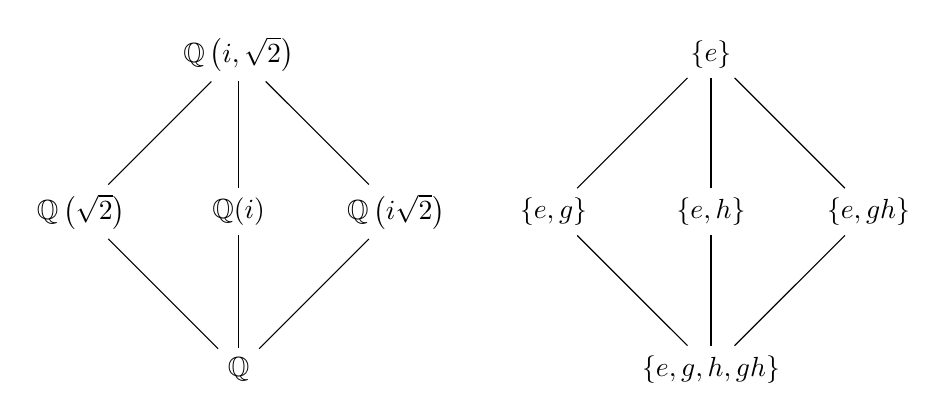
\begin{tikzpicture}[node distance=2cm]
        \node (Q)                  {$\mathbb{Q}$};
        \node (Qi)  [above of=Q]   {$\mathbb{Q}(i)$};
        \node (Qi2) [right of=Qi]  {$\mathbb{Q}\left(i\sqrt{2}\right)$};
        \node (Q2)  [left of=Qi]   {$\mathbb{Q}\left(\sqrt{2}\right)$};
        \node (Q2i) [above of=Qi]  {$\mathbb{Q}\left(i, \sqrt{2}\right)$};
        \node (eg)  [right of=Qi2] {$\{e, g\}$};
        \node (egh) [right of=eg]  {$\{e, h\}$};
        \node (eh)  [right of=egh] {$\{e, gh\}$};
        \node (G)   [below of=egh] {$\{e, g, h, gh\}$};
        \node (e)   [above of=egh] {$\{e\}$};
        \draw (Q)   -- (Qi2);
        \draw (Q)   -- (Q2);
        \draw (Q)   -- (Qi);
        \draw (Qi2) -- (Q2i);
        \draw (Q2)  -- (Q2i);
        \draw (Qi)  -- (Q2i);
        \draw (G)   -- (eg);
        \draw (G)   -- (egh);
        \draw (G)   -- (eh);
        \draw (eg)  -- (e);
        \draw (egh) -- (e);
        \draw (eh)  -- (e);
    \end{tikzpicture}
\end{center}

The recipe for producing an intermediate subfield from a subgroup is to take the elements of $\Q\left(i, \sqrt{2}\right)$ which are fixed by all elements of the subgroup.
For instance, $\Q\left(i \sqrt{2}\right)$ is the field of elements fixed by both $e$ and $gh$.

This correspondence doesn't always work for all finite field extensions.  It works for Galois extensions.
In the correspondence, normal extensions correspond to normal subgroups.
In this example, all subgroups are normal and the extensions are normal.
We'll also prove the Primitive Element Theorem, which in the context of finite extensions of $\Q$ tells us that they are necessarily of the form $\Q(\alpha)$ for some $\alpha$, for instance $\Q(i, \sqrt{2}) = \Q(i + \sqrt{2})$.

\subsection{Review of GRM}
\begin{ndef}\hypertarget{def:algebraic}
    Suppose $K \leq L$ is a field extension. Take $\alpha \in L$ and define
    \begin{equation*}
        I_\alpha = \set{f \in K[t] | f(\alpha) = 0}
    \end{equation*}
    We say $\alpha$ is \textbf{algebraic} over $K$ if $I_\alpha \ne 0$.  Otherwise $\alpha$ is \textbf{transcendental}.
    We say $L$ is algebraic over $K$ if $\alpha$ is algebraic over $K$ for all $\alpha \in L$.
\end{ndef}

\begin{remark}
    We can see $I_\alpha$ is an ideal of $K[t]$ since it is the kernel of the ring homomorphism $K[t] \to L$ given by $f(t) \mapsto f(\alpha)$.
\end{remark}

\begin{eg}
    \leavevmode
    \begin{enumerate}[label=(\roman*)]
        \item $\sqrt{2}$ is \hyperlink{def:algebraic}{algebraic} over $\Q$
        \item $\pi$ is algebraic over $\Q$
    \end{enumerate}
\end{eg}

\begin{nlemma}\label{lem:1.5}
    Let $K \leq L$ be a \hyperlink{def:degreeOfFieldExt}{finite} \hyperlink{def:fieldExt}{field extension}. Then $L$ is \hyperlink{def:algebraic}{algebraic} over $K$.
\end{nlemma}

\begin{proof}
    Let $\abs{L:K}=n$, and take $\alpha \in L$. Consider $1, \alpha, \alpha^2, \dotsc, \alpha^n$, which must be linearly dependent in the $n$-dimensional $K$--vector space $L$.
    So, $\sum_{i=0}^n \lambda_i \alpha^i = 0$ for some $\lambda \in K$ not all zero, and hence $\alpha$ is a root of $f(t) = \sum_{i=0}^n \lambda_i t^i$, so $\alpha$ is \hyperlink{def:algebraic}{algebraic} over $K$.
    $\alpha$ was arbitrary, so $L$ is algebraic over $K$.
\end{proof}

\begin{ndef}\hypertarget{def:minimalPoly}
    The non-zero ideal $I_\alpha$ (where $\alpha$ is \hyperlink{def:algebraic}{algebraic} over $K$) is principal since $K[t]$ is a principal ideal domain.
    In particular, we can say $I_\alpha = (f_\alpha(t))$ where $f_\alpha(t)$ can be assumed to be monic.
    Such a monic $f_\alpha(t)$ is the \textbf{minimal polynomial} of $\alpha$ over $K$.
\end{ndef}

\begin{remark}
    Multiplication by $\alpha$ within the field $L$ gives a $K$--linear map $L \to L$, an automorphism (if $\alpha \ne 0$).  In GRM, we have seen the \hyperlink{def:minimalPoly}{minimal polynomial} of a linear map is unique.
\end{remark}

\begin{eg}\leavevmode
    \begin{enumerate}[label=(\roman*)]
        \item The minimal polynomial of $\sqrt{2}$ over $\Q$ is $t^2 - 2$.
        \item The minimal polynomial of $\sqrt{2}$ over $\R$ is $t - \sqrt{2}$.
    \end{enumerate}
\end{eg}

\begin{nlemma}\label{lem:1.7}
    Suppose $K \leq L$ is a \hyperlink{def:fieldExt}{field extension}, $\alpha \in L$ and $\alpha$ is \hyperlink{def:algebraic}{algebraic} over $K$.
    Then the \hyperlink{def:minimalPoly}{minimal polynomial} $f_\alpha(t)$ of $\alpha$ over $K$ is irreducible in $K[t]$ and $I_\alpha$ is a prime ideal.
\end{nlemma}

\begin{proof}
    Suppose $f_\alpha(t) = p(t) q(t)$. We aim to show $p(t)$ or $q(t)$ is a unit in $K[t]$.
    But $0 = f_\alpha(\alpha) = p(\alpha) q(\alpha)$, so $p(\alpha) = 0$ or $q(\alpha) = 0$, without loss of generality take $p(\alpha) = 0$, thus $p(t) \in I_\alpha$.
    But $I_\alpha=(f_\alpha(t))$, so $p(t) = f_\alpha(t) r(t)$, giving $f_\alpha(t) = f_\alpha(t) r(t) q(t)$ and so $r(t) q(t) = 1$ in $K[t]$, and $q(t)$ is a unit, as required.
    Recall from GRM that irreducible elements of $K[t]$ are prime and hence generate prime ideals of $K[t]$. So $I_\alpha$ is a prime ideal.
\end{proof}

\begin{ndef}\hypertarget{def:genField}
    Suppose $K\leq L$ is a \hyperlink{def:fieldExt}{field extension} and $\alpha \in L$.  $K(\alpha)$ is defined to be the smallest subfield of $L$ containing $K$ and $\alpha$.
    It's called the field \textbf{generated} by $K$ and $\alpha$.  We say that $L$ is a \textbf{simple extension} if $L = K(\beta)$ for some $\beta \in L$.

    Given $\alpha_1, \dotsc, \alpha_n \in L$, $K \leq L$.  $K(\alpha_1, \dotsc \alpha_n)$ is the smallest field containing $\alpha_1, \dotsc, \alpha_n$.
    It is the field generated by $K$ and $\alpha_1, \dotsc, \alpha_n$.

    On the other hand $K[\alpha]$ is the ring generated by $K$ and $\alpha$, in particular the image of $K[t]$ under the map $f(t) \mapsto f(\alpha)$.
\end{ndef}

% new lec (3)

\begin{nthm}\label{thm:1.9}
    Suppose $K \leq L$ is a \hyperlink{def:fieldExt}{field extension} and $\alpha \in L$ is \hyperlink{def:algebraic}{algebraic} over $K$.  Then
    \begin{enumerate}[label=(\roman*)]
        \item  $K(\alpha) = K[\alpha]$
        \item $\abs{K(\alpha) : K} = \deg f_\alpha(t)$ where $f_\alpha(t)$ is the \hyperlink{def:minimalPoly}{minimal polynomial} of $\alpha$ over $K$.
    \end{enumerate}
\end{nthm}

\begin{proof}
    \leavevmode
    \begin{enumerate}[label=(\roman*)]
        \item Clearly $K[\alpha] \leq K(\alpha)$. We aim to show that any non-zero element $\beta$ of $K[\alpha]$ is a unit, so $K[\alpha]$ is a field.

            By definition of $K[\alpha]$, $\beta = g(\alpha)$ for some $g(t) \in K[t]$.  Since $\beta = g(\alpha) \neq 0$, $g(t) \notin I_\alpha = (f_\alpha(t))$.  Thus $f_\alpha(t) \nmid g(t)$.
            From \cref{lem:1.7}, $f_\alpha(t)$ is irreducible and $K[t]$ is a PID, we know $\exists r(t), s(t) \in K[t]$ with $r(t) f_\alpha(t) + s(t) g(t) = 1$ in $K[t]$.
            Hence $s(\alpha) g(\alpha) = 1$ in $K[\alpha]$, and so $\beta = g(\alpha)$ is a unit as required.
        \item Let $n = \deg f_\alpha(t)$ We'll show that $T = \set{1, \alpha, \alpha^2, \dotsc, \alpha^{n-1}}$ is a $K$--vector space.

            Spanning: If $f_\alpha(t) = t^n + a_{n-1} t^{n-1} + \dots + a_0$ with $a_i \in K$, then $\alpha^n = -a_{n-1} \alpha^{n-1} - \dots - a_0$.
            This implies $\alpha^n$ is a linear combination of $\set{1, \alpha, \alpha^2, \dotsc, \alpha^{n-1}}$, and an easy induction shows that $\alpha^m$ for $m \geq n$ is likewise a linear combination of $\set{1, \alpha, \alpha^2, \dotsc, \alpha^{n-1}}$, so we have spanning.

            Linear independence: Suppose $\lambda_{n-1} \alpha^{n-1} + \dotsc + \lambda_0 = 0$.
            Let $g(t) = \lambda_{n-1} t^{n-1} + \dotsc + \lambda_0$.  Since $g(\alpha) = 0$, we have $g(t) \in I_\alpha = (f_\alpha(t)).$  So $g(t) = 0$ or $f_\alpha(t) \mid g(t)$.
            The latter is not possible since $\deg f_\alpha(t) > \deg g_\alpha(t)$ so $g(t) = 0$ in $K[t]$ and all the $\lambda_i$'s are zero.
    \end{enumerate}
\end{proof}

\begin{ncor}\label{cor:1.10}
    If $K \leq L$ is a \hyperlink{def:fieldExt}{field extension} and $\alpha \in L$, then $\alpha$ is \hyperlink{def:algebraic}{algebraic} over $K$ if and only if $K \leq K(\alpha)$ is \hyperlink{def:degreeOfFieldExt}{finite}.
\end{ncor}

\begin{proof}
    $\Rightarrow$ By \cref{thm:1.9}, $\abs{K(\alpha):K} = \deg f_\alpha(t) \leq \infty$.

    $\Leftarrow$ \Cref{lem:1.5}
\end{proof}

\begin{ncor}\label{cor:1.11}
    Let $K \leq L$ be a \hyperlink{def:fieldExt}{field extension} with \hyperlink{def:degreeOfFieldExt}{$\abs{L:K} = n$}. Let $\alpha \in L$, then $\deg f_\alpha(t) \mid n$.
\end{ncor}

\begin{proof}
    Use the \nameref{thm:towerLaw} on $K \leq K(\alpha) \leq L$.  We deduce that $\abs{K(\alpha):K}$ divides $\abs{L:K}$.  \Cref{thm:1.9}(ii) gives $\deg f_\alpha(t) = \abs{K(\alpha) : K}$.
\end{proof}

\subsection{Digression on (Non-)Constructibility}
Schedules mention `other classical problems' and we are now in a position to tackle some of these using \cref{cor:1.11}.

A classical question from Greek geometry concerns the existence or otherwise of constructions using ruler and compasses (where a ruler refers to a single unmarked straight edge).
If you're an expert you can divide a line betwen 2 points into arbitrarily many equal segments, you can bisect an angle, or you can produce parallel lines.
Given a polygon you can produce a square of the same area or double the area. However,
\begin{enumerate}
    \item You cannot duplicate the cube using ruler and compasses (given a cube you can't produce a cube of double the volume)
    \item You cannot trisect the angle $\pi/3$ using ruler and compasses.
    \item The circle cannot be squared using ruler and compasses (given a circle you can't construct a square of the same area)
\end{enumerate}

Assume we're given a set $P_0$ of points in $\R^2$, and we can formalise our operations.
\begin{itemize}[label={}, leftmargin=*]
    \item \textbf{Ruler operation} Draw a straight line through any two points in $P_0$.
    \item \textbf{Compass operation} Draw a circle with centre being a point in $P_0$ and radius the distance between a pair of points in $P_0$.
\end{itemize}

\begin{ndef}[\hypertarget{def:constructible}{Constructible}]
    The points of intersection of any two distinct lines or circles drawn using these operations are \textbf{constructible in one step} from $P_0$.
    More generally, a point $\vec{r} \in \R^2$ is \textbf{constructible} from $P_0$ if there is a finite sequence $\vec{r_1}, \vec{r_2}, \dotsc, \vec{r_n} = \vec{r}$ such that $\vec{r_i}$ is constructible in one step from $P_0 \cup \set{\vec{r_1}, \dotsc, \vec{r_{i-1}}}$.
\end{ndef}

\begin{exercise}
    Construct the midpoint of a line between two points.
\end{exercise}

Let $K_0$ be the subfield of $\R$ \hyperlink{def:genField}{generated} by $\Q$ and the co-ordinates of the points in $P_0$. Let $\vec{r_i} = (x_i, y_i)$ and set $K_i = K_{i-1} (x_i, y_i)$.

Thus $K_0 \leq K_1 \leq K_2 \leq \dots \leq K_m \leq \R$.

\begin{nlemma}\label{lem:1.13}
    $x_i, y_i$ are both roots in $K_i$ of quadratic polynomials in $K_{i-1}[t]$.
\end{nlemma}

\begin{proof}
    There are three cases for $\vec{r_i}$: line meets line, line meets circle, circle meets circle. We do the second case only here.
    \begin{center}
        \begin{tikzpicture}[scale=1]
            \tkzDefPoint[label=below:$A$](-0.5,1){A}
            \tkzDefPoint[label=below:$B$](3,2){B}
            \tkzDefPoint[label=below:$C$](0,0){C}

            \tkzDrawCircle[R, very thin](C, 2.5cm)
            \tkzDrawSegment[very thin, add=3cm and 1cm](A, B)

            \tkzInterLC[R](A,B)(C,2.5cm) \tkzGetPoints{X}{Y}
            \tkzLabelPoints[above left](X)
            \tkzLabelPoints[above](Y)

            \tkzDrawPoints[fill=black](A,B,C,X,Y)
            % \draw (0, 0) circle [radius=2];
            % \draw (-3, 0) -- (3, 2);
        \end{tikzpicture}
    \end{center}
    The line is defined by two points $A = (p, q)$ and $B = (r, s)$ while the circle is defined with a centre $C = (t, u)$ and radius $w$.
    Then, points $X$ and $Y$ satisfy the equation of the line $\frac{x-p}{r-p} = \frac{y-q}{s-q}$, and the equation of the circle $(x-t)^2 + (y-u)^2 = w^2$.
    Solving these together gives coordinates of $X$ and $Y$ satisfying quadratic polynomials over $K_{i-1}$.
    The other two cases are left as an exercise for the reader.
\end{proof}

% new lec (4)

\begin{nthm}\label{thm:1.14}
    If $\vec{r} = (x, y)$ is constructible from a set $P_0$ of points in $\R^2$ and if $K_0$ is the subfield of $\R$ generated by $\Q$ and the coordinates of the points in $P_0$, then the degrees $\abs{K_0(x) : K_0}$ and $\abs{K_0(y):K_0}$ are powers of two.
\end{nthm}

\begin{proof}
    Continue with the previous notation of $K_i = K_{i-1}(x_i, y_i)$. By the \nameref{thm:towerLaw},
    \begin{equation*}
        \abs{K_i : K_{i-1}} = \abs{K_{i-1} (x, y): K_{i-1}(x)} \abs{K_{i-1}(x) : K_{i-1}}
    \end{equation*}
    But \cref{lem:1.13} tells us that $\abs{K_{i-1}(x):K_{i-1}}$ must be $1$ or $2$ depending on whether the quadratic polynomial arising in the lemma is reducible or not, using \cref{thm:1.9}(ii). Similarly, $\abs{K_{i-1}(x, y):K_{i-1}(x)}$ is 1 or 2.

    So $\abs{K_i: K_{i-1}} = 1, 2 \ \text{or} \ 4$, (but in fact $4$ cannot happen), hence by the \nameref{thm:towerLaw}, $\abs{K_n:K_0} = \abs{K_n:K_{n-1}} \abs{K_{n-1} : K_{n-2}} \dots \abs{K_1:K_0}$ is a power of two.

    If $r = (x, y)$ is constructible from $P_0$, then
    \begin{align*}
        x, y \in K_n \quad \text{and} \quad K_0 \leq &K_0(x) \leq K_n \\
        K_0 \leq &K_0(y) \leq K_n
    \end{align*}
    and the Tower Law again gives that $|K_0(x):K_0|$ and $|K_0(y):K_0|$ are also powers of $2$.
\end{proof}

To use this for proofs about non-constructibility we need to be reasonably expert at working out \hyperlink{def:minimalPoly}{minimal polynomials}.

\begin{nthm}\label{thm:1.15}
    Let $f(t)$ be a primitive integral polynomial.  Then $f(t)$ is irreducible in $\Q[t]$ if and only if it is irreducible in $\Z[t]$.
\end{nthm}

\begin{proof}
    A special case of Gauss' lemma from GRM.
\end{proof}

\begin{nthm}[Eisenstein's criterion]\label{thm:1.16}
    Let $f(t) = a_n t^n + a_{n-1} t^{n-1} + \dots + a_0 \in \Z[t]$.
    Suppose there is a prime $p$ such that
    \begin{enumerate}[label=(\roman*)]
        \item $p \nmid a_n$
        \item $p \mid a_{n-1}, \, p \mid a_{n-2}, \dotsc, p \mid a_0$
        \item $p^2 \nmid a_0$
    \end{enumerate}
    Then $f(t)$ is irreducible in $\Z[t]$
\end{nthm}

\begin{proof}
    Recall from GRM.
\end{proof}

\begin{eg}
    For $p$ a prime, consider $f(t) = t^{p-1} + t^{p-2} + \dots + 1$.  This is irreducible over $\Q$ by considering $f(t+1)$ and using $p$ as the prime in \nameref{thm:1.16}.
\end{eg}

Another method is to consider an integral polynomial $f(t) \pmod{p}$. If $f(t)$ is irreducible in $\Z[t]$ then it is reducible over $\Z / p \Z$. So, if we find a prime $p$ such that $f(t) \pmod{p}$ is irreducible then $f(t)$ is irreducible in $\Z[t]$.

\begin{eg}
    $t^3 + t + 1$ is irreducible mod $2$. If it were reducible it would have a linear factor and so the polynomial would have a root mod 2. But $0, 1$ are not roots. So, $t^3 + t + 1$ is irreducible in $\Z[t]$, hence irreducible in $\Q[t]$.
\end{eg}

\begin{remark}
    On a later example sheet you'll meet an irreducible polynomial in $\Z[t]$ which is reducible mod $p$ for all primes $p$.
\end{remark}

% back to non-constructibility
\begin{nthm}\label{thm:1.17}
    The cube cannot be duplicated by ruler and compasses.
\end{nthm}

\begin{proof}
    The problem amounts to whether given a unit distance, one can construct points distance $\alpha$ apart, where $\alpha$ satisfies $t^3 - 2 = 0$.
    Starting with points $P_0 = \{(0, 0), (1, 0)\}$ can we produce $(\alpha, 0)$?

    No. If we could, \cref{thm:1.14} would say $\abs{\Q(\alpha):\Q}$ is a power of 2. But $\abs{\Q(\alpha): \Q} = 3$ since $\abs{\Q(\alpha):\Q} = \deg f_\alpha(t)$ where $f_\alpha(t)$ is the \hyperlink{def:minimalPoly}{minimal polynomial} of $\alpha$ over $\Q$. $\alpha$ satisfies $t^3 - 2$, which is irreducible over $\Z$ by \nameref{thm:1.16} hence irreducible over $\Q$. So $t^3 - 2$ is the minimal polynomial $f_\alpha(t)$.
\end{proof}

\begin{nthm}\label{thm:1.18}
    The circle cannot be squared using ruler and compasses.
\end{nthm}

\begin{proof}
    Starting with $(0, 0)$ and $(1, 0)$, we must \hyperlink{def:constructible}{construct} $(\sqrt{\pi}, 0)$ so that we have a square of side length $\sqrt{\pi}$ and hence area $\pi$.
    But $\pi$ and hence $\sqrt{\pi}$ is transcendental over $\Q$ (Lindemann - not proved here).
    \Cref{thm:1.14} tells us we can't do this construction.
\end{proof}

\subsection{Return to theory development}
\begin{nlemma}\label{lem:1.19}
    Let $K \leq L$ be a \hyperlink{def:fieldExt}{field extension}. Then
    \begin{enumerate}[label=(\roman*)]
        \item $\alpha_1, \dotsc, \alpha_n \in L$ are \hyperlink{def:algebraic}{algebraic} over $K$ if and only if $K \leq K(\alpha_1, \dotsc \alpha_n)$ is a field extension.
        \item If $K \leq M \leq L$ such that $K \leq M$ is \hyperlink{def:degreeOfFieldExt}{finite}, then there exist $\alpha_1, \dotsc \alpha_n \in L$ such that $K(\alpha_1, \dotsc \alpha_n) = M$.
    \end{enumerate}
\end{nlemma}

\begin{proof}
    \leavevmode
    \begin{enumerate}[label=(\roman*)]
        \item By \cref{cor:1.10}, $\alpha$ is algebraic over $K$ if and only if $K \leq K[\alpha]$ is a \hyperlink{def:degreeOfFieldExt}{finite} field extension.
            $\alpha_i$ is algebraic over $K$ and hence algebraic over $K(\alpha_1, \dotsc \alpha_{i-1})$ and so
            $\abs{K(\alpha_1, \dotsc, \alpha_i):K(\alpha_1, \dotsc, \alpha_{i-1})} < \infty$.
            By the \nameref{thm:towerLaw} applied to $K \leq K(\alpha_1) \leq K(\alpha_1, \alpha_2) \leq \dots \leq K(\alpha_1, \dotsc \alpha_n)$, we get $\abs{K(\alpha_1, \dotsc \alpha_n):K} < \infty$

            Conversely, consider $K \leq K(\alpha_1) \leq K(\alpha_1, \dotsc \alpha_n)$.
            Then the tower law says that if $\abs{K(\alpha_1, \dotsc, \alpha_n): K} < \infty$ then $\abs{K(\alpha_1):K} < \infty$ and by \cref{cor:1.10}, $\alpha$ is algebraic over $K$.

        \item If $\abs{M:K} = n$ then $M$ is an $n$-dimensional $K$-vector space, so there exists a $K$-basis $\alpha_1, \dotsc, \alpha_n$ over $M$.
            Then $K(\alpha_1, \dotsc, \alpha_n) \leq M$.
            However, any element of $M$ is a $K$-linear combination of $\alpha_1, \dotsc, \alpha_n$ and so lies in $K(\alpha_1, \dotsc, \alpha_n)$, so $M = K(\alpha_1, \dotsc, \alpha_n)$.
    \end{enumerate}
\end{proof}

% new lec (5)

\begin{ndef}\hypertarget{def:homo}
    Suppose $K \leq L$, $K \leq L'$ are \hyperlink{def:fieldExt}{field extensions}. A \textbf{K-homomorphism} $\phi: L \to L'$ is a ring homomorphism such that $\phi\vert_K = \id$.

    A $K$-homomorphism is a $K$-isomorphism if it is a ring isomorphism.
\end{ndef}

\begin{notation}\hypertarget{not:hom}{}
    $ \Hom_K(L, L') = \{K\text{-homomorphisms} \; L \to L'\} $
\end{notation}

\begin{notation}
    \hypertarget{not:aut}{
    $ \Aut_K(L) = \{K\text{-isomorphisms} \; L \to L\} $
    } and note $\Aut_K(L)$ is a group
\end{notation}

\begin{nlemma}\label{lem:1.21}
    Suppose $K \leq L$, $K \leq L'$ are \hyperlink{def:fieldExt}{field extensions}. Then
    \begin{enumerate}[label=(\roman*)]
        \item Any \hyperlink{def:homo}{$K$-homomorphism} $\phi:L \to L'$ is injective and $K \leq \phi(L)$ is a field extension.
        \item If $|L:K| = |L':K| < \infty$ then any $K$-homomorphism $\phi:L \to L'$ is a \hyperlink{def:homo}{$K$-isomorphism}.
    \end{enumerate}
\end{nlemma}

\begin{proof}
    \leavevmode
    \begin{enumerate}[label=(\roman*)]
        \item $L$ is a field and $\ker \phi$ is an ideal of $L$.

            Note $1 \to 1$ and so $\ker \phi$ can't be the whole of $L$, hence $\ker \phi = \{0\}$ so $\phi(L)$ is a field and $K \leq \phi(L)$ is a field extension.
        \item $\phi$ is an injective $K$-linear map, so $|\phi(L):K| = |L:K|$. In general, $|\phi(L):K| \leq |L':K|$, but since $|L:K| = |L':K|$ by assumption, we have $|\phi(L):K| = |L':K|$, hence $\phi(L) = L'$ and $\phi$ is a $K$-isomorphism $L \to L'$.  (If $L' = L$ then $\phi$ would be a $K$-automorphism also.)
    \end{enumerate}
\end{proof}

\begin{notation}
    If $K \leq L$ is a \hyperlink{def:fieldExt}{field extension} and $f(t) \in K[t]$, we denote the set of roots of $f$ in $L$ by $\Root_f(L)$.
\end{notation}

\begin{ndef}\label{def:1.22}\hypertarget{def:splitting}
    Let $K \leq L$ be a field extension and $f(t) \in K[t]$. We say \textbf{$f$ splits over $L$} if
    \begin{equation*}
        f(t) = a (t-\alpha_1) (t - \alpha_2) \dotsm (t - \alpha_n)
    \end{equation*}
    where $a \in K$ and $\alpha_1, \dotsc, \alpha_n \in L$.

    We say $L$ is a \textbf{splitting field for $f$ over $K$} if $L = K(\alpha_1, \dotsc, \alpha_n)$.
\end{ndef}

\begin{remark}
    This is equivalent to saying that $L$ is a \hyperlink{def:splitting}{splitting field} for $f$ over $K$ iff
    \begin{enumerate}[label=(\roman*)]
        \item $f$ splits over $L$
        \item if $K \leq M \leq L$ and $f$ splits over $M$ then $M=L$.
    \end{enumerate}
\end{remark}

\begin{eg}
    \leavevmode
    \begin{enumerate}
        \item Consider $f(t) = t^3 - 2$ over $\Q$.

            $\Q(\sqrt[3]{2})$ is \emph{not} a \hyperlink{def:splitting}{splitting field} for $f$ over $\Q$, but $\Q(\sqrt[3]{2}, \omega\sqrt[3]{2}, \omega^2\sqrt[3]{2})$ is a splitting field over $\Q$ where $\omega$ is a primitive cube root of unity $\omega = e^{2\pi i/3}$
            \begin{center}
                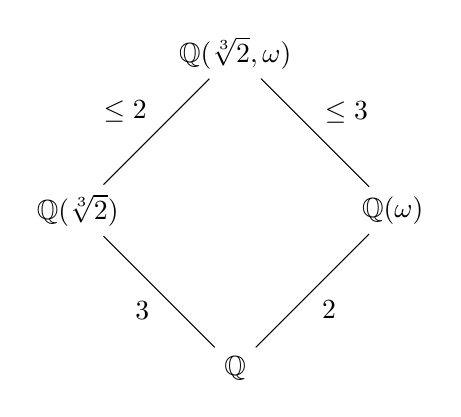
\begin{tikzpicture}[node distance=2cm]
                    \node (blank)                  {};
                    \node (Q2)    [left of=blank]  {$\Q(\sqrt[3]{2})$};
                    \node (Qw)    [right of=blank] {$\Q(\omega)$};
                    \node (Q)     [below of=blank] {$\Q$};
                    \node (Qw2)   [above of=blank]  {$\Q(\sqrt[3]{2}, \omega)$};

                    \draw (Qw2) -- (Qw)  node[midway,anchor=south west]{$\leq 3$}
                                -- (Q)   node[midway,anchor=north west]{$2$}
                                -- (Q2)  node[midway,anchor=north east]{$3$}
                                -- (Qw2) node[midway,anchor=south east]{$\leq 2$};
                \end{tikzpicture}
            \end{center}

            Starting in the bottom right, going clockwise:
            \begin{itemize}
                \item The \hyperlink{def:minimalPoly}{minimal polynomial} of $\omega$ over $\Q$ is $t^2 + t + 1$, so $\abs{\Q(\omega):\Q}=2$.
                \item $t^3 - 2$ is irreducible over $\Q$ by \nameref{thm:1.16}, so $\abs{\Q(\sqrt[3]{2}):\Q}=3$.
                \item $\omega$ satisfies $t^2 + t + 1$ over $\Q$ and hence over $\Q(\sqrt[3]{2})$ and so $\abs{\Q(\sqrt[3]{2}, \omega):\Q(\sqrt[3]{2})} \leq 2$.
                \item $\sqrt[3]{2}$ satisfies $t^3 - 2$ over $\Q$ and hence over $\Q(\omega)$, so $\abs{\Q(\sqrt[3]{2}, \omega):\Q(\omega)} \leq 3$.
            \end{itemize}

            Then by the \nameref{thm:towerLaw}, $2 \mid \abs{\Q(\sqrt[3]{2}, \omega): \Q}$ and $3 \mid \abs{\Q(\sqrt[3]{2}, \omega): \Q}$, so we deduce
            \begin{align*}
                \abs{\Q(\sqrt[3]{2}, \omega) : \Q(\omega)} = 3 \\
                \abs{\Q(\sqrt[3]{2}, \omega) : \Q(\sqrt[3]{2})} = 2
            \end{align*}

        \item Take $f(t) = (t^2 - 3)(t^3 - 1)$. The splitting field for $f$ over $\Q$ is
            \begin{align*}
                &\Q(\sqrt{3}, -\sqrt{3}, \omega, \omega^2, 1) \\
                = &\Q(\sqrt{3}, \omega) = \Q(\sqrt{3}, i)
            \end{align*}
            since $\omega = \frac{-1 + i \sqrt{3}}{2}$.
        \item $t^2 - 3$ and $t^2 - 2t - 2$ have the same splitting field over $\Q$: $\Q(\sqrt{3})$
        \item Take $f(t) = t^2 + t + 1$ in $\mathbb{F}_2[t]$.

            $f(t)$ is irreducible over $\mathbb{F}_2$ since it has no roots in $\mathbb{F}_2$ and hence no linear factors in $\mathbb{F}_2[t]$.
            Hence, $\mathbb{F}_2[t]/(t^2 + t + 1)$ is a field.

            Set $\alpha = t + (t^2 + t + 1) \in \mathbb{F}_2[t]/(t^2 + t + 1)$, then
            \begin{equation*}
                \frac{\mathbb{F}_2[t]}{(t^2 + t + 1)} = \mathbb{F}_2[\alpha]
            \end{equation*}

            The elements are $0, 1, \alpha, 1+\alpha$ noting that $\alpha^2 + \alpha + 1 = 0$ and since we have characteristic $2$, $\alpha^2 = \alpha + 1$.

            $f(t)$ splits over $\mathbb{F}_2[\alpha]$:
            \begin{equation*}
                f(t) = (t-\alpha)(t-1-\alpha)
            \end{equation*}
            Thus $\mathbb{F}_2[\alpha]$ is the splitting field for $f$ over $\mathbb{F}_2$.
    \end{enumerate}
\end{eg}
We can use this final construction to produce splitting fields in general.

\begin{nthm}[Existence of splitting fields]\label{thm:1.23}
    Let $K$ be a field and $f(t) \in K[t]$. Then there exists a \hyperlink{def:splitting}{splitting field} for $f$ over $K$.
\end{nthm}

\begin{proof}
    If $\deg f = 0$ then $K$ is the splitting field for $f$ over $K$.

    Suppose $\deg f > 0$ and pick an irreducible factor $g(t)$ of $f(t)$ in $K[t]$, noting that $K \leq K[t] / (g(t))$ is a \hyperlink{def:fieldExt}{field extension}.

    Take $\alpha_1 = t + (g(t)) \in K[t]/(g(t))$, then $K[t]/(g(t)) = K(\alpha_1)$ and $g(\alpha_1) = 0$ in $K(\alpha_1)$.
    Therefore $f(\alpha_1) = 0$ in $K(\alpha_1)$ and we can write $f(t) = (t-\alpha_1) h(t)$ in $K(\alpha_1)[t]$.

    Repeat, noting that $\deg h(t) < \deg f(t)$ and so we get $f(t) = a(t - \alpha_1)(t - \alpha_2) \dotsm (t-\alpha_n)$ where $a$ is a constant in $K$.
    Thus, we have a factorisation of $f(t)$ in $K(\alpha_1, \dotsc, \alpha_n)[t]$, and so $K(\alpha_1, \dotsc, \alpha_n)$ is a splitting field for $f$ over $K$.
\end{proof}

\begin{nthm}[Uniqueness of splitting fields]\label{thm:1.24}
    If $K$ is a field and $f(t) \in K[t]$, then the \hyperlink{def:splitting}{splitting field} for $f$ over $K$ is unique up to \hyperlink{not:hom}{$K$-isomorphism}, that is, if there are two such splitting fields $L$ and $L'$, there is a $K$-isomorphism $\phi: L \to L'$.
\end{nthm}

% new lec (6)

\begin{proof}
    Suppose $L$ and $L'$ are splitting fields for $f(t) \in K[t]$ over $K$. We need to show that there is a $K$-isomorphism $L \to L'$.

    Suppose $K \leq M \leq L$ and there exist $M'$ with $K \leq M' \leq L'$ and a $K$-isomorphism $\psi: M \to M'$.
    Clearly some $M$ exists (we can take $M=K$), so we pick $M$ so that $\abs{M:K}$ is maximal among all such $M, M', \psi$.

    We must show $M=L$ and $M' = L'$. Note that if $M = L$ then $f(t)$ splits over $M$:
    \begin{equation*}
        f(t) = a(t - \alpha_1) \dotsm (t - \alpha_n) \in M[t]
    \end{equation*}
    Apply $\psi$, we get an induced map $M[t] \to M'[t]$.
    \begin{equation*}
        f(t) = \psi(f(t)) = \psi(a) (t - \psi(\alpha_1)) \dotsm (t - \psi(\alpha_n))
    \end{equation*}
    Thus $f(t)$ splits over $\psi(M) = M'$. But $L'$ is a splitting field and $M' \leq L'$, so $M'=L'$.

    So, suppose $M\neq L$ and we'll get a contradiction of maximality of $M$.
    Since $M \neq L$, there is a root $\alpha$ of $f(t)$ in $L$ which isn't in $M$.
    Factorise $f(t) = g(t) h(t)$ in $M[t]$ so that $g(t)$ is irreducible in $M[t]$ while $g(\alpha) = 0$ in $L$.
    Then there exists a $K$-homomorphism $M[t]/(g(t)) \to L$ given by $t + (g(t)) \mapsto \alpha$ which has image $M(\alpha)$.

    The $K$-isomorphism $M[t] \to M'[t]$ induced by $\psi$ maps $g(t) \in M[t]$ to $\gamma(t) \in M'[t]$.
    $f(t) = g(t) h(t)$ in $M[t]$ yields $f(t) = \gamma(t) \delta(t)$ in $M'[t]$.

    We have a field extension $M' \leq M'[t]/(\gamma(t))$ and there exists a $M'$-homomorphism $M'[t]/(\gamma(t)) \to L'$ given by $t + (\gamma(t))$ by picking a root $\alpha'$ of $\gamma(t)$ in $L'$.
    However $\gamma(t) \mid f(t)$ in $M'[t]$ and hence in $L'[t]$ and so $\alpha'$ is also a root of $f(t)$ in $L'$.
    The $M'$-homomorphism gives a $K$-isomorphism
    \begin{equation*}
        M'[t] / (\gamma(t)) \to M'(\alpha')
    \end{equation*}
    and so we have a $K$-isomorphism $M(\alpha) \to M'(\alpha')$. This contradicts the maximality of $M$, since $M \lneqq M(\alpha)$.
\end{proof}

\begin{ndef}[Normal extension]\label{def:1.25}\hypertarget{def:normal}
    A \hyperlink{def:fieldExt}{field extension} $K \leq L$ is \textbf{normal} if for every $\alpha \in L$ the \hyperlink{def:minimalPoly}{minimal polynomial} $f_\alpha(t)$ of $\alpha$ over $K$ \hyperlink{def:splitting}{splits} over $L$.
\end{ndef}

\begin{nthm}\label{thm:1.26}
    Let $K \leq L$ be a \hyperlink{def:degreeOfFieldExt}{finite} \hyperlink{def:fieldExt}{field extension}. Then $K \leq L$ is \hyperlink{def:normal}{normal} $\iff$ $L$ is the \hyperlink{def:splitting}{splitting field} for some $f(t) \in K[t]$.
\end{nthm}

\begin{proof}
    Later.
\end{proof}

\begin{nexample}\label{thm:1.27}
    Let $\F$ be a finite field with $\abs{\mathbb{F}} = m$. $\F$ has characteristic $p$ for some $p$ and $\F_p \leq \F$, therefore $m = p^r$ for some $r$.
    The non-zero elements form the multiplicative group of order $m-1=n$ and they satisfy $t^n - 1$: they are roots of $t^n - 1$. So,
    \begin{equation*}
        t^n - 1 = (t - \alpha_1) \dotsm (t-\alpha_n)
    \end{equation*}
    where $\alpha_1, \dotsc, \alpha_n$  are the non-zero elements of $\F$. Thus $\F$ is the splitting field for $t^n - 1$ over $\F_p$.
    By \cref{thm:1.24}, any other field with $m$ elements is $\F_p$-isomorphic to $\F$.
    (We'll show later that there is a field of $M$ elements.)
\end{nexample}

\begin{nthm}\label{thm:1.28}
    Let $G$ be a finite subgroup of the multiplicative group of a field $K$. Then $G$ is cyclic. In particular, the multiplicative group of a finite field is cyclic.
\end{nthm}

\begin{proof}
    Let $\abs{G} = n$. By the structure theorem of finite abelian groups from GRM,
    \begin{equation*}
        G \cong C_{q_1^{m_1}} \times C_{q_2^{m_2}} \times \dotsm \times C_{q_r^{m_r}}
    \end{equation*}
    with $q_i$ prime, not necessarily distinct.
    However if $q = q_i = q_j$ for some $i \neq j$, there are at least $q^2$ distinct solutions of $t^q - 1 = 0$ in $K$ (since $C_q \times C_q \cong$ subgroup of $G$).
    But in a field (or even an integral domain), a polynomial of degree $q$ has at most $q$ roots, a contradiction.
    So all the $q_i$ are distinct and hence $G$ is cyclic, generated by $(g_1, \dotsc, g_r)$ where $g_i$ generates $C_{q_i^{m_i}}$ using the Chinese Remainder Theorem.
\end{proof}

\clearpage

\section{Separable, normal and Galois extensions}

\begin{ndef}[Separable polynomial]\hypertarget{def:separablePoly}
    Let $K$ be a field and $f(t) \in K[t]$. Suppose $f(t)$ is irreducible in $K[t]$ and $L$ is a splitting field for $f(t)$ over $K$.
    Then $f(t)$ is \textbf{separable} over $K$ if $f(t)$ has no repeated roots in $L$.

    For general $f(t)$ we say $f(t)$ is separable over $K$ if every irreducible factor in $K[t]$ is separable over $K$.

    All constant polynomials are separable.
\end{ndef}

% new lec (7)

\begin{ndef}[Formal differentiation]\hypertarget{def:diff}
    If $K$ is a field then \textbf{formal differentiation} $D: K[t] \to K[t]$ is a $K$-linear map with $D(t^n) = n t^{n-1}$.
    We denote this by $D(f(t)) = f'(t)$.
\end{ndef}

\begin{nlemma}\label{lem:2.3}
    Let $K$ be a field and $f(t), g(t) \in K[t]$. Then:
    \begin{enumerate}[label=(\alph*)]
        \item $D(f(t) g(t)) = f'(t) g(t) + f(t) g'(t)$ (Leibniz' rule)
        \item Assume $f(t) \neq 0$. Then $f(t)$ has a repeated root in a splitting field $L$ if and only if $f(t)$ and $f'(t)$ have a common irreducible factor in $K[t]$.
    \end{enumerate}
\end{nlemma}

\begin{proof}
    \leavevmode
    \begin{enumerate}[label=(\alph*)]
        \item $D$ is a $K$-linear map and so we only need to check for $f(t) = t^n$, $g(t) = t^m$. Left as an exercise.
        \item Let $\alpha$ be a repeated root in a splitting field $L$, then
            \begin{align*}
                f(t) &= (t-\alpha)^2 g(t) \in L[t] \\
                f'(t) &= (t-\alpha)^2 g'(t) + 2(t-\alpha) g(t)
            \end{align*}
            and so $f'(\alpha) = 0$.
            Therefore the minimal polynomial $f_\alpha(t)$ of $\alpha$ in $K[t]$ divides both $f(t)$ and $f'(t)$ and thus $f_\alpha(t)$ is a common irreducible factor of $f(t)$ and $f'(t)$.


            Conversely, let $h(t)$ be a common irreducible factor of $f(t)$ and $f'(t)$ in $K[t]$.
            Pick a root $\alpha$ in $L$ of $h(t)$.

            So $f(\alpha) = 0 = f'(\alpha)$, Thus $f(t) = (t-a) g(t)$ in $L[t]$, and $f'(t) = (t-a) g'(t) + g(t)$.

            Since $f'(\alpha)  = 0$ we have $(t-a) \mid f'(t)$. and so $(t-a) \mid g(t)$. Hence $(t-a)^2 \mid f(t)$ and we have a repeated root.
    \end{enumerate}
\end{proof}

\begin{ncor}\label{cor:2.4}
    If $K$ is a field and $f(t) \in K[t]$ is irreducible:
    \begin{enumerate}[label=(\roman*)]
        \item If the characteristic of $K$ is 0, then $f(t)$ is separable over $K$.
        \item If the characteristic of $K$ is greater than 0, then $f(t)$ is not separable if and only if $f(t) \in K[t^p]$.
    \end{enumerate}
\end{ncor}

\begin{proof}
    By \cref{lem:2.3}, $f(t)$ is not separable over $K$ if and only if $f(t)$ and $f'(t)$ have a common ireeducible factor.
    Since we're assuming $f(t)$ is irreducible, this is equivalent to saying $f'(t) = 0$.

    \begin{align*}
        f(t) &= a_n t^n + a_{n-1} t^{n-1} + \dotsb + a_0 \\
        f'(t) &= n a_n t^{n-1} + \dotsb + a_1
    \end{align*}
    Thus $f'(t) = 0 \iff i a_i = 0$ for all $i > 0$.

    \begin{enumerate}[label=(\roman*)]
        \item If $\chara K = 0$ then $f'(t) \neq 0$ for non-constant polynomials, so $f(t)$ is separable over $K$.
        \item If $\chara K = p > 0$ then if $f'(t) = 0$ we have $i a_i = 0$ for all $i > 0$, so $f(t)$ is not separable $\iff f(t) \in K[t^p]$.
    \end{enumerate}
\end{proof}

\begin{ndef}[Separable extension]\hypertarget{def:separableExt}
    We say \textbf{$\alpha \in L$ is separable over $K$} if its \hyperlink{def:minimalPoly}{minimal polynomial} is \hyperlink{def:separablePoly}{separable} over $K$.

    \textbf{$L$ is separable over $K$} if all $\alpha \in L$ are separable over $K$.

    If $f_\alpha(t) = (t-\alpha)^n = t^n - \alpha^n$ where $n$ is a power of $p (=\chara K)$, we say that $\alpha$ is \textbf{purely inseparable over $K$}.
\end{ndef}

\begin{eg}
    \leavevmode
    \begin{enumerate}[label=(\arabic*)]
        \item Let $\Q \subseteq L$ be an \hyperlink{def:algebraic}{algebraic} \hyperlink{def:fieldExt}{field extension}. Then $L$ is \hyperlink{def:separablePoly}{separable} over $K$.
        \item Let $L = \F_p(X)$ be the rational functions in $X$ over $\F_p$, and $K = \F_p(X^p)$.
            Then $K \leq L$ is not separable. Observe that if $f(t) = t^p - X^p \in K[t]$ then $f'(t) = 0$. But $t^p - X^p = (t-X)^p$ in $L[t]$ since the binomial expansion other terms divisible by $p$ and hence $0$ since the characteristic is $p$.

            However $f(t)$ is irreducible in $K[t]$:

            Suppose $f(t) = g(t) h(t)$ in $K[t]$ and hence in $L[t]$. So we get $g(t) = (t-X)^r$ for some $0 \leq r < p$ if the factorisation is non-trivial.
            But this would mean $X^r$ was in $K$. However, $\exists$integers $a, b$ such that $ar + bp = 1$.
            So $(X^r)^a (X^p)^b \in K$ and so $X \in K$, thus we'd have $X = \frac{u(X^p)}{v(X^p)}$, a contradiction.

            Thus $f(t) = t^p - X^p$ is the \hyperlink{def:minimalPoly}{minimal polynomial} of $X$ over $K$, thus $X$ is \hyperlink{def:separableExt}{purely inseparable} over $K$ and $K \leq L$ is not separable.
        \item Take $\F$ a finite field with order $m$, a power of $p$ where $\chara \F = p$. Consider $f(t) = t^n - 1$ where $n = m-1$. This is separable over $\F_p$ since we saw that $f(t)$ has distinct linear factors in $\F[t]$.
    \end{enumerate}
\end{eg}

\begin{remark}
    It's useful to have an alternative approach to \hyperlink{def:separableExt}{separability of field extensions} without having to check \hyperlink{def:separablePoly}{separability}
    of \hyperlink{def:minimalPoly}{minimal polynomials} for all elements of the larger field.
    This is where we start thinking about \hyperlink{def:homo}{$K$-homomorphisms}.
\end{remark}

\begin{nlemma}\label{lem:2.6}
    Let $M = K(\alpha)$, where $\alpha$ is \hyperlink{def:algebraic}{algebraic} over $K$ and let $f_\alpha(t)$ be the \hyperlink{def:minimalPoly}{minimal polynomial} of $\alpha$ over $K$.

    Then, for any \hyperlink{def:fieldExt}{field extension} $K \leq L$, the number of \hyperlink{def:homo}{$K$-homomorphisms} of $M$ to $L$ is equal to the number of distinct roots of $f_\alpha(t)$ in $L$.
    Thus this number is $\leq \deg f_\alpha(t) = \abs{K(\alpha):K} = \abs{M:K}$.

    \begin{center}
        \begin{tikzpicture}[scale=0.8]
            \node (K) at ( 0,-2)    {$K$};
            \node (L) at ( 2, 2)    {$L$};
            \node (M) at (-2, 0)    {$M = K(\alpha)$};

            \draw (M) -- (K) -- (L);
        \end{tikzpicture}
    \end{center}
\end{nlemma}

\begin{proof}
    We saw in \cref{lem:1.21} that any $K$-homomorphism $M \to L$ is injective, and we have
    \begin{equation*}
        K(\alpha) \cong \frac{K[t]}{(f_\alpha(t))}.
    \end{equation*}
    For any root $\beta$ of $f_\alpha(t)$ in $L$ we can define a $K$-homomorphism
    \begin{align*}
        \frac{K[t]}{(f_\alpha(t))} &\to L \\
        t + (f_\alpha(t)) &\mapsto \beta
    \end{align*}
    Thus we get a $K$-homomorphism $M \to L$.

    Conversely, for any $K$-homomorphism $\phi:M \to L$ the image $\phi(\alpha)$ must satisfy
    \begin{equation*}f_\alpha(\phi(\alpha)) = 0\end{equation*}
    These processes are inverse to each other, giving a 1-1 correspondence
    \begin{equation*}
        \{K \text{ homomorphisms } M \to L\} \longleftrightarrow \{\text{roots of } f_\alpha(t) \in L\}
    \end{equation*}
\end{proof}

% new lec (8)

\begin{eg}
    Take $K = \Q$, $L = \Q(\sqrt[3]{2})$, and use $\alpha = \sqrt[3]{2}$, with \hyperlink{def:minimalPoly}{minimal polynomial} $f_\alpha(t) = t^3 - 2$.

    Then, there is only one \hyperlink{def:homo}{$K$-homomorphism} $M = K(\sqrt[3]{2})  =L \to L$, the identity map.
\end{eg}

\begin{ncor}\label{cor:2.7}
    % TODO understand this corollary
    The number of $K$-homomorphisms $K(\alpha) \to L = \deg f_\alpha(t) \iff L$ is large enough, in particular $L$ contains a splitting field for $f_\alpha(t)$ and $\alpha$ is separable over $K$.
\end{ncor}

\begin{proof}
    Immediate from \cref{lem:2.6}.
\end{proof}

\begin{nlemma}\label{lem:2.8}
    Let $K \leq M$ be a field extension and $M_1 = M(\alpha_1)$ (where $\alpha_1$ is algebraic over $M$).
    Let $f(t)$ be the minimal polynomial of $\alpha$ over $M$ and let $K \leq L$.
    Let $\phi: M \to L$ be a $K$-homomorphism. Then there is a correspondence
    \begin{equation*}
        \{\text{Extensions } \phi_1:M_1 \to L \text{ of } \phi\} \longleftrightarrow \{\text{roots of} \ \phi(f(t)) \in L\}
    \end{equation*}
    \begin{center}
        \begin{tikzpicture}
            \node (K)  at ( 0,-2)    {$K$};
            \node (M)  at (-1, -0.5)    {$M$};
            \node (M1) at (-2, 1)    {$M_1$};
            \node (L)  at ( 2, 2)    {$L$};

            \draw (M1) -- (M) -- (K) -- (L);
        \end{tikzpicture}
    \end{center}
\end{nlemma}

\begin{remark}
    \Cref{lem:2.6} is the special case $M=K$ and $\phi =$ inclusion of $K$ in $L$.
\end{remark}

\begin{proof}
    $f(t)$ is irreducible in $M[t]$, so $\phi(f(t))$ is irreducible in $\phi(M)[t]$.
    Any extension $\phi_1: M \to L$ of $\phi$ produces a root $\phi_1(\alpha_1)$ of $\phi(f(t))$.

    Conversely, given a root $\gamma$ of $\phi(f(t))$ in $L$,
    \begin{equation*}
        M_1 - M(\alpha_1) \cong \frac{M[t]}{(f(t))} \cong \frac{\phi(M)[t]}{(\phi(f(t)))} \cong \phi(M)(\phi) \leq L
    \end{equation*}
    Thus we get an extension $\phi_1$ of $\phi$ as required.
\end{proof}

\begin{ncor}\label{cor:2.9}
    If $L$ is large enough, the number of $\phi_1$ which extend $\phi$ is equal to the number of distinct roots of $f(t)$ in $L$. This is equal to $|M_i:M| \iff \alpha$ is separable over $M$.
\end{ncor}

\begin{proof}
    Immediate from \cref{lem:2.8}.
\end{proof}

\begin{ncor}\label{cor:2.10}
    Let $K \leq M \leq N$ be finite field extensions, $K \leq L$. Let $\phi: M \to L$ be a $K$-homomorphism.
    Then the number of extensions of $\phi$ to maps $\theta:N \to L$ is $\leq \abs{N:M}$.
    Moreover, such a $\theta$ exists if $L$ is large enough.
\end{ncor}

\begin{proof}
    Pick $\alpha_1, \dotsc, \alpha_r$ so that $N = M(\alpha_1, \dotsc, \alpha_r)$ and set $M_i = M(\alpha_1, \dotsc,\alpha_i)$. Then we've got
    \begin{equation*}
        M \leq M_1 \leq M_2 \leq \dotsb \leq M_r = N.
    \end{equation*}

    Using \cref{lem:2.8}, there are
    \begin{align*}
        \leq& \abs{M_1:M} \text{ extensions } \phi_1 : M_1 \to L \text{ of } \phi \\
        \leq& \abs{M_2:M_1} \text{ extensions } \phi_2 : M_2 \to L \text{ of } \phi \\
        &\vdots \\
        \leq& \abs{M_r:M_{r-1}} \text{ extensions } \phi_r : M_r \to L \text{ of } \phi
    \end{align*}
    By the \nameref{thm:towerLaw}, the number of extensions $\theta: N \to L$ (recall $N=M_r$) of $\phi:M \to L$ is
    \begin{equation*}
        \leq \abs{M_r:M_{r-1}} \abs{M_{r-1}:M_{r-2}} \cdots \abs{M_1:M} = \abs{N:M}
    \end{equation*}
    where the last part comes from the proof of \cref{lem:2.8} - we need $L$ to contain roots.
\end{proof}

\begin{nremark}\label{rem:2.11}
    This proof together with \cref{cor:2.9} shows that the number of extensions $\theta$ of $\phi$ is equal to $\abs{N:M}$ iff $L$ is large enough (so that everything splits) and $\alpha_i$ is separable over $M(\alpha_1, \dotsc, \alpha_{i-1})$.
\end{nremark}

\begin{nlemma}\label{lem:2.12}
    Let $K \leq N$ be a field extension with $\abs{N:K} = n$ and $N = K(\alpha_1, \dotsc, \alpha_r)$ say.
    Then the following are equivalent:
    \begin{enumerate}[label=(\roman*)]
        \item $N$ is separable over $K$.
        \item Each $\alpha_i$ is separable over $K(\alpha_1, \dotsc, \alpha_n)$.
        \item If $K \leq L$ is large enough there are exactly $n$ distinct $K$-homomorphisms $N \to L$.
    \end{enumerate}
\end{nlemma}

\begin{proof}
    (i) $\Rightarrow$ (ii).
    $N$ is separable over $K \implies  \alpha_i$ is separable over $K$.
    The \hyperlink{def:minPoly}{minimal polynomial} of $\alpha_i$ over $K(\alpha_1, \dotsc, \alpha_{i-1})$ divides the minimal polynomial of $\alpha_i$ over $K$ (in $K(\alpha_1, \dotsc, \alpha_{i-1})[t]$).

    So if the latter has distinct roots in a splitting field then the former does.
    So $\alpha_i$ separable over $K \implies \alpha_i$ separable over $K(\alpha_1, \dotsc, \alpha_{i-1})$.

    (ii) $\Rightarrow$ (iii) follows from \cref{rem:2.11}.

    (iii) $\Rightarrow$ (i). Assume (iii) is false and (i) true, aiming for a contradiction.
    So, $\exists \beta \in N$ that is not \hyperlink{def:separableExt}{separable} over $K$, so there are $\lneqq\abs{K(\beta):K}$ $K$-homomorphisms $\phi:K(\beta) \to L$ by \cref{cor:2.7}.

    By \cref{cor:2.10}, $\phi$ extends to $\leq \abs{N:K(\beta)}$ extensions $\theta: N \to L$, and so there are $\lneqq\abs{N:K(\beta)}\abs{K(\beta):K}$ $K$-homomorphisms $N\to L$, contradiction.
\end{proof}

\begin{ndef}[Separably generated]\label{def:2.13}\hypertarget{def:separableGen}
    We say $M = K(\alpha_1, \dotsc, \alpha_r)$ is \textbf{separably generated} by $\alpha_1, \dotsc, \alpha_r$ over $K$ if each $\alpha_i$ is separable over $K$.
\end{ndef}

\begin{ncor}\label{cor:2.14}
    A finite extension is \hyperlink{def:separableExt}{separable} $\iff$ it is \hyperlink{def:separableGen}{separably generated}.
\end{ncor}

\begin{proof}
    As already observed, $\alpha_i$ is separable over $K \implies  \alpha_i$ separable over $K(\alpha_1, \dotsc, \alpha_{i-1})$.
\end{proof}

\begin{nlemma}\label{lem:2.15}
    If $K \leq M \leq L$ \hyperlink{def:degreeOfFieldExt}{finite} \hyperlink{def:fieldExt}{field extensions}, $M \leq L$, then
    \begin{equation*}
        K \leq M, \; \; M \leq L \text{ are both separable } \iff K \leq L \text{ is separable}
    \end{equation*}
\end{nlemma}

\begin{proof}
    Example sheet.
\end{proof}

\begin{nexample}
    Take $\F$ a finite field, $\abs{\F} = m$. Multiplicative group of order $n = m - 1$ is cyclic.
    Take a generated $\alpha$, then $\F = \F_p(\alpha)$, and so the \hyperlink{def:minimalPoly}{minimal polynomial} of $\alpha$ divides $t^n - 1$.
    Observe this has distinct roots, which are all of $\F \setminus \{0\}$ since $\alpha^n = 1$.
    So the minimal polynomial of $\alpha$ is \hyperlink{def:separablePoly}{separable}, and $\F = \F_p(\alpha)$ is separable over $\F_p$.
\end{nexample}

% new lec (9)

\begin{nthm}\label{thm:2.17}
    Any finite separable extension $K \leq M$ is a simple extension, that is, $M = K(\alpha)$ for some $\alpha$ a primitive element.
\end{nthm}

\begin{proof}
    First deal with the case where $K$ is a finite field. Then $M$ is also finite and we can take $\alpha$ to be a generator of the multiplicative group of $M$, which is cyclic.

    Now assume $K$ is an infinite field.

    Since $K\leq M$ is a finite extension, $M = K(\alpha_1, \alpha_2, \dotsc, \alpha_n)$ for some $\alpha_i$.
    It is enough to show that any field $M = K(\alpha, \beta)$ with $\beta$ separable over $K$ is of the form $K(\gamma)$.

    Take $f(t)$ and $g(t)$ to be the minimal polynomials of $\alpha$ and $\beta$ over $K$ and let $L$ be the splitting field for $f(t) g(t)$ over $K(\alpha, \beta)$.
    The distinct zeros of $f(t)$ in $L$ are $\alpha = \alpha_1, \dotsc, \alpha_a$ and of $g(t)$ are $\beta = \beta_1, \dotsc, \beta_b$.

    By separability, $b = \deg g(t)$.
    Choose $\lambda \in K$ such that all $\alpha_i + \lambda \beta_j$ are distinct, which is possible since $K$ is infinite.
    Set $\gamma = \alpha + \lambda \beta$.

    Let $F(t) = f(\gamma - \lambda t) \in K(\gamma)[t]$. We have $g(\beta) = 0$ and $F(\beta) = f(\alpha) = 0$. Thus $F(t)$ and $g(t)$ have a common zero.

    Any other common zero would have to be $\beta_j$ for some $j > 1$. But then $F(\beta_j) = f(\alpha + \lambda(\beta - \beta_j))$.
    By assumption, $\alpha + \lambda(\beta - \beta_j)$ is never an $\alpha_i$ and so $F(\beta_j) \neq 0$.
    Separability of $g(t)$ says its linear factors are all distinct, so $(t-\beta)$ is a highest common factor of $F(t)$ and $g(t)$ in $L[t]$.

    However the minimal polynomial $h(t)$ of $\beta$ over $K(\gamma)$ then divides $F(t)$ and $g(t)$ in $K(\gamma)[t]$ and hence in $L[t]$. This implies $h(t) = t - \beta$ and so $\beta \in K(\gamma)$.
    Therefore $\alpha = \gamma - \lambda \beta \in K(\gamma)$ and so $K(\alpha, \beta) \subset K(\gamma)$ and equality holds since $\gamma \in K(\alpha, \beta)$.
\end{proof}

\begin{eg}
    From our example in (link) chapter 1, $\Q \leq \Q(\sqrt{2}, i)$, we had intermediate subfields.
    \begin{center}
        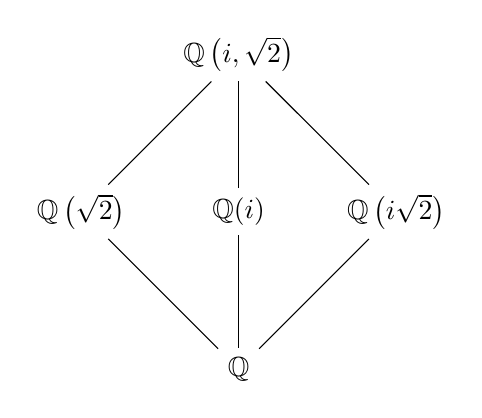
\begin{tikzpicture}[node distance=2cm]
            \node (Q)                  {$\mathbb{Q}$};
            \node (Qi)  [above of=Q]   {$\mathbb{Q}(i)$};
            \node (Qi2) [right of=Qi]  {$\mathbb{Q}\left(i\sqrt{2}\right)$};
            \node (Q2)  [left of=Qi]   {$\mathbb{Q}\left(\sqrt{2}\right)$};
            \node (Q2i) [above of=Qi]  {$\mathbb{Q}\left(i, \sqrt{2}\right)$};
            \draw (Q)   -- (Qi2);
            \draw (Q)   -- (Q2);
            \draw (Q)   -- (Qi);
            \draw (Qi2) -- (Q2i);
            \draw (Q2)  -- (Q2i);
            \draw (Qi)  -- (Q2i);
        \end{tikzpicture}
    \end{center}
    If we follow the procedure of the proof of \cref{thm:2.17}, $\alpha = \sqrt{2}$, $\beta = i$, $f(t) = t^2 - 2$, $g(t) = t^2 + 1$.
    Consider $\sqrt{2} + \lambda i$ where $\pm \sqrt{2} \pm \lambda i$ are distinct.
    For instance $\lambda = 1$, so $\Q(\sqrt{2}, i) = \Q(\sqrt{2}+i)$.
\end{eg}

\subsection{Trace and Norm}

\begin{ndef}[Trace and norm]\label{def:2.18}\hypertarget{def:trNorm}
    Let $K \leq M$ be a finite field extension, and $\alpha \in M$. Multiplication by $\alpha$ gives a $K$-linear map $\theta_\alpha: M \to M$.

    Then we define
    \begin{itemize}[label={}]
        \item \textbf{Trace of $\alpha$ over $K$} is given by $\Tr_{M/K}(\alpha) =$ trace of $\theta_\alpha$  $\in K$.
        \item \textbf{Norm of $\alpha$ over $K$} is given by $N_{M/K}(\alpha) =$ determinant of $\theta_\alpha$  $\in K$.
    \end{itemize}

    Note these are dependent on the field extension.
\end{ndef}

\begin{nthm}\label{thm:2.19}
    With the above notation, suppose $f_\alpha(t) = t^s + a_{s-1} t^{s-1} + \dotsb + a_0$ is the minimal polynomial for $\alpha$ over $K$.
    Let $r = \abs{M:K(\alpha)}$, then the characteristic polynomial of $\theta_\alpha$ is $(f_\alpha(t))^r$.

    Note $\abs{M:K} = \abs{M:K(\alpha)} |K(\alpha) : K| = rs$.
    Then $\Tr_{M/K} (\alpha) = -r a_{s-1}$ and $N_{M/K} = ((-1)^s a_0)^r$.
\end{nthm}

\begin{proof}
    Regard $M$ as a $K(\alpha)$-vector space with basis $1 = \beta_1, \dotsc, \beta_r$.
    Now take the $K$-vector space basis $1, \alpha, \alpha^2, \dotsc, \alpha^{s-1}$ of $K(\alpha)$.
    So, $1, \alpha, \alpha^2, \dotsc, \alpha^{s-1}, \beta_2, \beta_2 \alpha, \dotsc, \beta_2 \alpha^{s-1}, \beta_3, \dotsc$ is a $K$-vector space basis for $M$.
    Multiplication by $\alpha$ in $K(\alpha)$ is represented by matrix
    \begin{equation*}
        A =
        \begin{pmatrix}
            0      & 0      & 0      & \dots  & 0      & -a_0     \\
            1      & 0      & 0      & \dots  & 0      & -a_1     \\
            0      & 1      & 0      & \dots  & 0      & -a_2     \\
            0      & 0      & 1      & \dots  & 0      & -a_3     \\
            \vdots & \vdots & \vdots & \ddots & \vdots & \vdots   \\
            0      & 0      & 0      & \dots  & 1      & -a_{s-1}
        \end{pmatrix}
    \end{equation*}
    an $s \times s$ matrix whose characteristic polynomial is $f_\alpha(t)$.

    Multiplication by $\alpha$ in $M$ is represented by the $rs \times rs$ matrix
    \begin{equation*}
        10 %stuff
    \end{equation*}
    whose characteristic polynomial is $(f_\alpha(t))^r$.

    Look at the terms of this characteristic polynomial to get the trace and norm.
\end{proof}

\begin{nthm}\label{thm:2.20}
    Let $K \leq M$ be a finite separable field extension and $|M:K| = n$, $\alpha \in M$.
    Let $K \leq L$ be large enough so that there are $n$ distinct $K$-homomorphisms
    \begin{equation*}
        \sigma_1, \sigma_2, \dotsc, \sigma_n: M \longrightarrow L.
    \end{equation*}
    Then the characteristic polynomial of $\theta_\alpha:M \to M_\alpha$ (the multiplication map) is
    \begin{equation*}
        \prod_{i=1}^n (t-\sigma_i(\alpha))
    \end{equation*}
    hence
    \begin{equation*}
        \Tr_{M/K} (\alpha) = \sum_{i=1}^n \sigma_i(\alpha) \qquad \text{and} \qquad N_{M/K}(\alpha) = \prod_{i=1}^n \sigma_i(\alpha).
    \end{equation*}
\end{nthm}

\begin{proof}
    $f_\alpha(t) = (t-\alpha_1) \dotsc (t-\alpha_s)$ in $L[t]$
    $ = t^s + a_{s-1} t^{s-1} + \dotsc + a_0$
    minimal polynomial of $\alpha$ over $K$.
    (where $L$ large enough implies $f_\alpha(t)$ splits in $L$).
    There are $s$ $K$-homomorphisms $K[\alpha] \to L$ corresponding to maps sending $\alpha$ to $\alpha_i$.

    Each of these extends in $\abs{M:K(\alpha)}$ ways to give $K$-homomorphisms $M \to L$. (by separability and 2.9).


    However each such extension of a map sending $\alpha \to \alpha_i$ still sends $\alpha \to \alpha_i$.
    Set $r = |L:K(\alpha)|$. Thus there are $r$ maps sending $\alpha \to \alpha_i$ for each $i$.
    Thus if the $n (=rs)$ distinct $K$-homomorphisms $M \to L$ are $\sigma_1, \dotsc, \sigma_n$, then
    \begin{align*}
        \sum_{i=1}^n \sigma_i(\alpha) &= r(\alpha_1 + \alpha_2 + \dotsb + \alpha_s) = -r a_{s-1} = \Tr_{M/K}(\alpha) \\
        \prod_{i=1}^n \sigma_i(\alpha) &= ((-1)^s a_0)^n = N_{M/K}(\alpha)
    \end{align*}
\end{proof}

% new lec (10)

\begin{nthm}\label{thm:2.21}
    Let $K \leq M$ be a finite \hyperlink{def:separableExt}{separable extension}.
    Then we define a $K$-bilinear form
    \begin{align*}
        T: M \times M &\rightarrow K \\
        (x, y) &\longmapsto \Tr_{M/K} (xy).
    \end{align*}

    Then this is non-degenerate and in particular the $K$-linear map $\Tr_{M/K}:M \to K$ is non-zero, and hence surjective.
\end{nthm}

\begin{remark}
    If $K \leq M$ is a finite extension which is not \hyperlink{def:separableExt}{separable} then $\Tr_{M/K}: M \to K$ is always zero and so $T:M\times M \to K$ is degenerate (see example sheet).
\end{remark}

\begin{proof}
    Separability and finiteness gives $M=K(\alpha)$ for some $\alpha$, by \cref{thm:2.17}.
    We have a $K$-basis $1, \alpha, \alpha^2, \dotsc, \alpha^{n-1}$ of $K(\alpha)$ where $n = \abs{M:K}$.
    The $K$-bilinear form is represented by
    \begin{equation*}
        A =
        \begin{pmatrix}
            \Tr_{M/K}(1)      & \Tr_{M/K}(\alpha)   & \dots  \\
            \Tr_{M/K}(\alpha) & \Tr_{M/K}(\alpha^2) & \dots  \\
            \vdots            & \vdots              & \ddots \\
        \end{pmatrix}.
    \end{equation*}
    Let $L$ be the splitting field of the minimal polynomial $f_\alpha(t)$ of $\alpha$ over $K$.

    Thus $f_\alpha(t) = (t-\alpha_1) \dotsm (t-\alpha_n)$ with $\alpha_1, \dotsc, \\alpha_n \in L$.
    The entries in $A$ are of the form $\Tr_{M/K}(\alpha^e)$ which is $\alpha_1^e + \dotsb \alpha_n^e$ using \cref{thm:2.20}.

    Now consider $\Delta = \prod_{i < j} (\alpha_i - \alpha_j)$, the discriminant of $V$:
    \begin{equation*}
        V =
        \begin{pmatrix}
            1 & 1 & \dots & 1 \\
            a_1 & a_2 & \dots & a_n \\
            a_1^2 & a_2^2 & \dots & a_n^2 \\
            \vdots & \vdots & \ddots & \vdots \\
            a_1^{n-1} & a_2^{n-1} & \dots & a_n^{n-1}
        \end{pmatrix}.
    \end{equation*}
    Observe that $V V^T = A$, and $0 \neq \Delta^2 = \abs{V V^T} = \abs{A}$, so $A$ is non-singular and therefore the bilinear form $T$ is non-degenerate.
\end{proof}

\begin{remark}
    We'll meet $\Delta$ again shortly, as it is the discriminant of the polynomial $f_\alpha(t)$.
\end{remark}

\subsection{Normal extensions}
We restate \cref{def:1.25} and \cref{thm:1.26}:

\begin{manual}{Definition 1.25}[Normal extension]
    An \hyperlink{def:fieldExt}{extension} $K \leq L$ is \textbf{normal} if for every $\alpha \in L$ the \hyperlink{def:minimalPoly}{minimal polynomial} $f_\alpha(t)$ of $\alpha$ over $K$ \hyperlink{def:splitting}{splits} over $L$.
\end{manual}

\begin{manual}{Theorem 1.26}
    Let $K \leq L$ be a \hyperlink{def:degreeOfFieldExt}{finite} \hyperlink{def:fieldExt}{field extension}. Then $K \leq L$ is \hyperlink{def:normal}{normal} $\iff$ $L$ is the \hyperlink{def:splitting}{splitting field} for some $f(t) \in K[t]$.
\end{manual}

\begin{proof}
    Assume $K \leq M$ is normal. Pick $\alpha_1, \dotsc, \alpha_r \in M$ so that $M = K(\alpha_1, \dotsc, \alpha_r)$.
    Let $f_{\alpha_i}(t)$ be the minimal polynomial for $\alpha_i$ over $K$.

    Let $f(t) = f_{\alpha_1}(t) f_{\alpha_2}(t)  \dotsc f_{\alpha_r}(t)$.
    By normality, each $f_{\alpha_i}(t)$ splits over $M$ and therefore $f(t)$ splits over $M$.
    $M$ is the splitting field of $f(t)$ over $K$ since if $\beta_1, \dotsc, \beta_m$ are the roots of $f(t)$ then $M=K(\beta_1, \dotsc, \beta_m)$.

    Conversely, suppose $M$ is a splitting field for $f(t)$ over $K$. Thus $M= K(\beta_1, \dotsc, \beta_m)$ where the $\beta_j$ are the roots of $f(t)$ in $M$.

    Take $\alpha\in M$. Let $f(t)$ be the minimal polynomial of $\alpha$ over $K$.
    Let $M \leq L$ large enough so that $f_\alpha(t)$ splits in $L$ and consider $K$-homomorphisms $\phi:M \to L$.

    $\phi(\beta_j)$ is also a root of $f(t)$ and is therefore one of the $B_j$s. Injectivity of $K$-homomorphisms (1.21) implies that $\phi$ generate the $\beta_j$.

    However $M = K(\beta_1, \dotsc, \beta_m)$ and so $\phi$ is determined by the images of the $\beta_j$ and thus $\phi(M) = M$.
    However if $\alpha_i$ is a root of $f_\alpha(t)$ in $L$, there is a $K$-homomorphism
    \begin{align*}
        K(\alpha) \to K(\alpha_i) \leq L \\
        \alpha \mapsto \alpha_i
    \end{align*}
    This extends by \cref{cor:2.10} to a $K$ homomorphism $\phi: M \to L$ with $\phi(\alpha) = \alpha_i$.
    But $\phi(M) = M$, so $\alpha_i \in M$. Thus $M$ is normal over $K$.
\end{proof}

\begin{remark}
    As for separability, the property of `normality' is equivalent to `normally generated'.
    In particular, a finite extension $K \leq L$ is normal if and only if $L = K(\alpha_1, \dotsc, \alpha_r)$, with each $f_{\alpha_i}(t)$ splitting over $L$.
\end{remark}

\begin{ndef}[Automorphism group]\label{def:2.22}\hypertarget{def:autGroup}
    Let $K \leq M$ be a finite field extension.
    Its \textbf{$K$-automorphism} group is $\Aut_K(M) = \set{\phi | \phi \text{ a $K$-homomorphism } M \to M}$.
\end{ndef}

From \cref{lem:1.21} we know that such $K$-homomorphisms are isomorphisms and thus have inverses. Composition gives the group operation.

\begin{nlemma}\label{lem:2.23}
    \begin{equation*}
        \Aut_K(M) \leq \abs{M:K}
    \end{equation*}
\end{nlemma}

\begin{proof}
    \Cref{cor:2.10}.
\end{proof}

\begin{nthm}\label{2.24}
    Let $K \leq M$ be a finite field extension. Then $\Aut_K(M) = \abs{M:K} \iff$ the extension is both normal and separable.
\end{nthm}

\begin{ndef}[Galois extension]\label{def:2.25}\hypertarget{def:galois}
    A finite field extension that is normal and separable is a \textbf{Galois extension}.
\end{ndef}
\end{document}
